\documentclass[a4paper]{scrreprt}

%% Language and font encodings
\usepackage[german]{babel}
\setcounter{secnumdepth}{3} 
\setcounter{tocdepth}{3} 
\usepackage[utf8x]{inputenc}
\usepackage[T1]{fontenc}
\usepackage{courier}

%% Sets page size and margins
\usepackage[a4paper,top=3cm,bottom=2cm,left=3cm,right=3cm,marginparwidth=1.75cm]{geometry}

%% Useful packages
\usepackage{amsmath}
\usepackage{graphicx}
\usepackage[colorinlistoftodos]{todonotes}
\usepackage[colorlinks=true, allcolors=blue, breaklinks = true]{hyperref}
\usepackage{tocstyle}
\usetocstyle{standard}
\settocfeature{raggedhook}{\raggedright}
\usepackage{longtable}
\usepackage{scrhack}
\usepackage{graphicx}
\usepackage{float}
\graphicspath{ {images/} }

\begin{document}	
	\begin{flushright}
		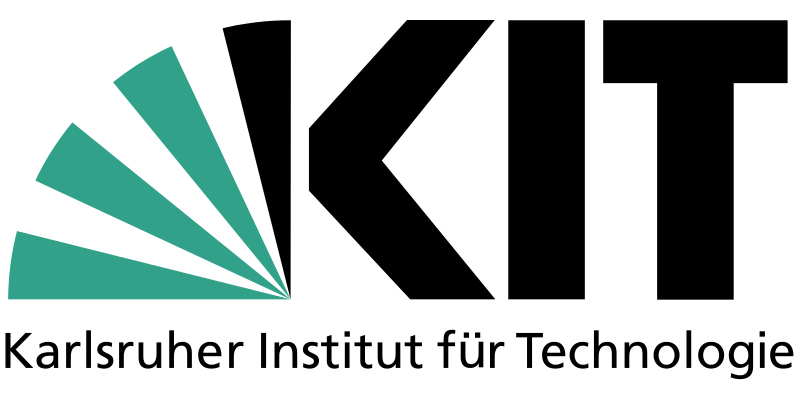
\includegraphics[scale = 0.2]{kit-logo.png}\\[0.5cm]
	\end{flushright}
	\vspace*{2cm}
	
	\begin{center}
		\large Praxis der Softwareentwicklung
		\vspace*{1.5cm}
		
		\textbf{\huge Fridget}
		\vspace*{1cm}
		
		\textbf{\Large Implementierung}
		\vspace*{2cm}
		
		Yunjia Chen, Jasmin Jat, Min Hye Park, Alina Shah, Lisa Wang
		\vspace*{1cm}
		
		\today
		\vspace*{2.5cm}
		
		Betreuung: Erik Burger, Sandro Koch\\[0.5cm]
		IPD\\[0.5cm]
		
		Karlsruher Institut für Technologie
		
	\end{center}

	\thispagestyle{empty}
	
	\tableofcontents
	
	\chapter{Einleitung}
	Dies ist das Dokument für die Implementierung der Applikation Fridget – entstanden im Rahmen
	des Softwarepraktikums PSE im Sommersemester 2018.
	Zunächst verlieren wir in diesen Dokument Worte über die Umsetzung von den Muss- und Wunschkriterien unserer App.
	In Abschnitt 3 beschreiben wir die Änderungen gegenüber des Feinentwurfs.
	Die Änderungen gegenüber der Datenstruktur wird in Abschnitt 4 erläutert.
	Ebenso wichtig sind die Unit Tests der Applikation, welche im nachfolgenden Abschnitt 5 aufgelistet sind.
	Um Fachbegriffe zu erläutern, befindet sich im letzten Abschnitt ein Glossar.
	
	\chapter{Umsetzung von den Muss- und Wunschkriterien}
	\section{Umgesetzte Musskriterien}
		\begin{table}[h!]
			\centering
			\label{my-label}
			\begin{tabular}{p{2cm}p{12cm}}
				
				\multicolumn{2}{c}{\textbf{1 - Erstellen einer WG-Pinnwand}} \\ \hline
				\centering{[}KM1010{]} & Eine Person muss sich in der App mit einem Google Account registrieren.\\
				\centering{[}KM1020{]}& Ein Benutzer kann sich mit einem Zugangscode bei einer bestehenden WG-Pinnwand anmelden oder eine neue WG-Pinnwand erstellen.                                 \\
				\centering{[}KM1030{]}& Beim Erstellen einer neuen WG-Pinnwand gibt der Benutzer dieser einen Namen.\\ 
				\centering{[}KM1040{]}& Die Pinnwand ist unterteilt in \textit{Frozen Notes} und \textit{Cool Notes}.\\ 
				\centering{[}KM1050{]}& Die \textit{Frozen Notes} sind feste, nicht löschbare, bearbeitbare Notizen und werden beim Erstellen der WG generiert.\\ 
				\centering{[}KM1060{]}& Die \textit{Cool Notes} sind löschbare, nicht bearbeitbare Notizen und werden vom Benutzer erstellt.\\ 
				\hline
			\end{tabular}
		\end{table}
		
		\vspace{5mm}
		
		\begin{table}[h!]
			\centering
			\label{my-label}
			\begin{tabular}{p{2cm}p{12cm}}
				
				\multicolumn{2}{c}{\textbf{2 - Interaktion mit der Pinnwand}} \\ \hline
				\centering{[}KM2010{]} & Der Benutzer kann eine \textit{Cool Note} mit einer Überschrift und Textinhalt erstellen und löschen.\\
				\centering{[}KM2020{]}& Der Benutzer kann die \textit{Frozen Notes} bearbeiten.                                 \\
				\centering{[}KM2030{]}& Dem Benutzer wird eine Magnetfarbe zugeteilt.\\ 
				
				\hline
			\end{tabular}
		\end{table}
		
		\vspace{5mm}
		
		\begin{table}[h!]
			\centering
			\label{my-label}
			\begin{tabular}{p{2cm}p{12cm}}
				
				\multicolumn{2}{c}{\textbf{3 - Synchronisierung mit dem Server}} \\ \hline
				\centering{[}KM3010{]} & Der Benutzer kann die App manuell aktualisieren.\\
				
				\hline
			\end{tabular}
		\end{table}
		
		\vspace{5mm}
		
		\begin{table}[h!]
			\centering
			\label{my-label}
			\begin{tabular}{p{2cm}p{12cm}}
				
				\multicolumn{2}{c}{\textbf{4 - App-Menü}} \\ \hline
				\centering{[}KM4010{]} & Der Benutzer kann eine Liste der Mitglieder und ihre entsprechende Magnetfarbe einsehen.\\
				\centering{[}KM4020{]}& Der Benutzer kann eine WG verlassen.                               \\
				\centering{[}KM4030{]}& Die App-Sprache ist Englisch.\\ 
				
				\hline
			\end{tabular}
		\end{table}
		
		\vspace{5mm}
		
		\begin{table}[h!]
			\centering
			\label{my-label}
			\begin{tabular}{p{2cm}p{12cm}}
				
				\multicolumn{2}{c}{\textbf{5 - Lesebestätigung}} \\ \hline
				\centering{[}KM5010{]} & Der Ersteller sieht, wer seine \textit{Cool Notes} gelesen hat.\\
				\centering{[}KM5020{]}& Der Benutzer kann markieren, welche \textit{Cool Notes} er gelesen hat.                               \\ 
				
				\hline
			\end{tabular}
		\end{table}
		
		\vspace{5mm}
		
		\begin{table}[h!]
			\centering
			\label{my-label}
			\begin{tabular}{p{2cm}p{12cm}}
				
				\multicolumn{2}{c}{\textbf{6 - Push-Benachrichtigung}} \\ \hline
				\centering{[}KM5010{]} & Alle Mitglieder bekommen für eine neue \textit{Cool Note} eine Push-Benachrichtigung.\\
				\centering{[}KM5020{]}& Über die Push-Benachrichtigung gelangt der Benutzer direkt zur neuen \textit{Cool Note}.                               \\
				
				\hline
			\end{tabular}
		\end{table}
	\section{Umgesetzte Wunschkriterien}
	Wir konnten leider keine unserer Wunschkriterien in Fridget umsetzen. Unser Problem war großteils Zeit, da für uns die richtige Implementierung der Muss-Kriterien Vorrang hatten.\\
	Jedoch wurden die Wunschkriterien KW1010 und KW1020 (``Benutzer können nur in ihrer \textit{Cool Note} einen oder mehrere Mitglieder taggen." und ``Nur die getaggten Mitglieder bekommen eine Push-Benachrichtigung.") auf der Serverseite implementiert.\\
	
	\newpage
	
	\chapter{Änderungen gegenüber dem Feinentwurf}
	
	\section{Package edu.kit.pse.fridget.client.activity}
		\subsection{Entfernte Klassen}
			Die folgende Klassen wurden als Fragmente implementiert und daher wurden die Activity Klassen entfernt.
			\begin{itemize}
				\item \texttt{public GetAccessCodeActivity extends AppCompatActivity implements View.OnClickListener}
				\item \texttt{public class MemberListActivity extends AppCompatActivity implements View.OnClickListener implements SwipeRefreshLayout.OnRefreshListener}
			\end{itemize}
			Die folgende Klassen sind leere Klassen die noch nicht implementiert wurden, da sie für Wunschkriterien gebraucht sind.
			\begin{itemize}
				\item \texttt{public class FullImageCoolNoteActivity extends AppCompatActivity implements View.OnClickListener implements SwipeRefreshLayout.OnRefreshListener}
				\item \texttt{public class CreateImageCoolNoteActivity extends AppCompatActivity implements View.OnClickListener implements SwipeRefreshLayout.OnRefreshListener}
				\item \texttt{public class CreateCommentActivity extends AppCompatActivity implements View.OnClickListener}
				\item \texttt{public class LanguageActivity extends AppCompatActivity implements View.OnClickListener}
			\end{itemize}
		\subsection{\texttt{public class LoginActivity extends AppCompatActivity implements View.OnClickListener}}
			\textbf{Neue Methoden}
			\begin{itemize}
				\item \texttt{public void onStart()}
				\item \texttt{public void onActivityResult(int requestCode, int resultCode, Intent data)}
				\item \texttt{private void firebaseAuthWithGoogle}
				\item \texttt{public void onClick(View v)}
				\item \texttt{private void signIn()}
				\item \texttt{private void sendIdToken(String googleIdToken)}
				\item \texttt{private void updateUI()}
			\end{itemize}
		\subsection{\texttt{public class StartActivity extends AppCompatActivity implements View.OnClickListener}}
			\textbf{Neue Methoden}
			\begin{itemize}
				\item \texttt{protected void onStart()}
				\item \texttt{protected void onResume()}
				\item \texttt{protected void onPause()}
				\item \texttt{protected void onStop()}
				\item \texttt{protected void onDestroy()}
				\item \texttt{private void updateUI(String flatshareId())}
			\end{itemize}
		\subsection{\texttt{public class CreateFlatshareActivity extends AppCompatActivity implements View.OnClickListener}}
			\textbf{Neue Methoden}
			\begin{itemize}
				\item \texttt{protected void onStart()}
				\item \texttt{protected void onPause()}
				\item \texttt{protected void onStop()}
				\item \texttt{private void updateUI(String flatshareId())}
			\end{itemize}
		\subsection{\texttt{public class EnterAccessCodeActivity extends AppCompatActivity implements View.OnClickListener}}
			\textbf{Neue Methoden}
			\begin{itemize}
				\item \texttt{protected void onStart()}
				\item \texttt{protected void onPause()}
				\item \texttt{protected void onStop()}
				\item \texttt{private void updateUI(String flatshareId())}
			\end{itemize}
		\subsection{\texttt{public class HomeActivity extends AppCompatActivity implements View.OnClickListener implements SwipeRefreshLayout.OnRefreshListener } ersetzt durch \texttt{public class HomeActivity extends AppCompatActivity implements View.OnClickListener implements NavigationView.OnNavigationItemSelectedListener }}
			\textbf{Neue Methoden}
			\begin{itemize}
				\item \texttt{public boolean onOptionsItemSelected(MenuItem item)}
				\item \texttt{public boolean onNavigationItemSelected(MenuItem item)}
				\item \texttt{public void onBackPressed()}
				\item \texttt{protected void onStart()}
				\item \texttt{protected void onResume()}
				\item \texttt{protected void onPause()}
				\item \texttt{protected void onStop()}
				\item \texttt{protected void onDestroy()}
			\end{itemize}
		\subsection{\texttt{public class FullTextCoolNoteActivity extends AppCompatActivity implements View.OnClickListener implements SwipeRefreshLayout.OnRefreshListener} \textit{ersetzt durch} \texttt{public class FullTextCoolNoteActivity extends AppCompatActivity}}
			\textbf{Neue Methoden}
			\begin{itemize}
				\item \texttt{public boolean onOptionsItemSelected(MenuItem item)}
				\item \texttt{protected void onStart()}
				\item \texttt{protected void onResume()}
				\item \texttt{protected void onPause()}
				\item \texttt{protected void onStop()}
				\item \texttt{protected void onDestroy()}
			\end{itemize}
		\subsection{\texttt{public class FullFrozenNoteActivity extends AppCompatActivity implements View.OnClickListener implements SwipeRefreshLayout.OnRefreshListener} \textit{ersetzt durch} \texttt{public class FullTextFrozenNoteActivity extends AppCompatActivity}}
			\textbf{Neue Methoden}
			\begin{itemize}
				\item \texttt{public boolean onOptionsItemSelected(MenuItem item)}
				\item \texttt{protected void onStart()}
				\item \texttt{protected void onResume()}
				\item \texttt{protected void onPause()}
				\item \texttt{protected void onStop()}
				\item \texttt{protected void onDestroy()}
			\end{itemize}
		\subsection{\texttt{public class CreateTextCoolNoteActivity extends AppCompatActivity implements View.OnClickListener} \textit{ersetzt durch} \texttt{public class CreateTextCoolNoteActivity extends AppCompatActivity}}
			\textbf{Neue Methoden}
			\begin{itemize}
				\item \texttt{public boolean onOptionsItemSelected(MenuItem item)}
				\item \texttt{protected void onStart()}
				\item \texttt{protected void onResume()}
				\item \texttt{protected void onPause()}
				\item \texttt{protected void onStop()}
				\item \texttt{protected void onDestroy()}
			\end{itemize}
		\subsection{\texttt{public class EditFrozenNoteActivity extends AppCompatActivity implements View.OnClickListener} \textit{ersetzt durch} \texttt{public class EditTextFrozenNoteActivity extends AppCompatActivity}}
		\textbf{Neue Methoden}
		\begin{itemize}
			\item \texttt{public boolean onOptionsItemSelected(MenuItem item)}
			\item \texttt{protected void onStart()}
			\item \texttt{protected void onResume()}
			\item \texttt{protected void onPause()}
			\item \texttt{protected void onStop()}
			\item \texttt{protected void onDestroy()}
		\end{itemize}
		
		\subsection{\texttt{public class AccessCodeActivity extends AppCompatActivity implements View.OnClickListener} \textit{ersetzt durch} \texttt{public class AccessCodeActivity extends AppCompatActivity}}
		\textbf{Neue Methoden}
		\begin{itemize}
			\item \texttt{public boolean onOptionsItemSelected(MenuItem item)}
			\item \texttt{protected void onStart()}
			\item \texttt{protected void onResume()}
			\item \texttt{protected void onPause()}
			\item \texttt{protected void onStop()}
			\item \texttt{protected void onDestroy()}
		\end{itemize}
	
		\section{Package edu.kit.fridget.client.datamodel}
	\subsection{Entfernte Datamodels}
	\begin{itemize}
		\item \texttt{public class Notification}
	\end{itemize}
	\textbf{Begründung:}\\
	Wir haben kein Datamodel für die Push-Benachrichtigung gebraucht, da wir Firebase dafür benutzt haben.
	\subsection{Veränderte Datamodels}
	\subsubsection{\texttt{public class CoolNote}}
	\textbf{Entfernte Attribute}
	\begin{itemize}
		\item \texttt{String flatshareId}
	\end{itemize}
	\textbf{Begründung:}\\
	Wir haben die Cool Notes über die creatorMembershipId identifiziert und diese hängt mit der flatshareId zusammen. Daher war ein extra Attribut flatshareId nicht nötig.\\
	\textbf{Veränderte Attribute}
	\begin{itemize}
		\item \texttt{String creatorUserId -> String creatorMembershipId}
		\item \texttt{List<String> taggedUserIds -> List<String> taggedMembershipIds}
	\end{itemize}
	\textbf{Begründung:}\\
	User ist die falsche Bezeichnung. Innerhalb einer Flatshare wird ein User zu einem Member. Die Beziehung zwischen Flatshare und Member wird als Membership bezeichnet.
	\subsubsection{\texttt{public class ReadConfirmation}}
	\textbf{Veränderte Attribute}
	\begin{itemize}
		\item \texttt{String readConfirmationId -> String id}
		\item \texttt{String userId -> String membershipId}
	\end{itemize}
	\textbf{Begründung:}\\
	Da es die Id im Datamodel ReadConfirmation ist, braucht man das nicht extra im Namen erwähnen. Die userId wurde umbenannt, da innerhalb einer Flatshare ein User zu einem Member wird.
	\subsection{Neue Datamodels}
	\subsubsection{\texttt{public class Device}}
	\textbf{Beschreibung} \\
	\textit{Diese Klasse stellt ein Endgerät dar.} \\
	
	\textbf{Attribute}
	\begin{itemize}
		\item \textbf{id}: Die ID des Devices. \\
		\textbf{Typ:} String
		
		\item \textbf{userId:} Die ID des Users, dem das Device gehört. \\
		\textbf{Typ:} String
		
		\item \textbf{instanceIdToken:} Ein Token, der für die Push-Benachrichtigung benötigt wird.\\
		\textbf{Typ:} String
	\end{itemize}
	
	\textbf{Methoden}
	\begin{itemize}
		\item{\texttt{public String getUserId()}}\\
		\textit{Gibt die User-ID des Users als String zurück.}\\
		\item{\texttt{public String getInstanceIdToken()}}\\
		\textit{Gibt den InstanceID-Token als String zurück.}\\
	\end{itemize}
	\subsubsection{\texttt{public class CreateFlatshareCommand}}
	\textbf{Beschreibung} \\
	\textit{Die Klasse CreateFlatshareCommand stellt ein Model dar, das die richtigen Attribute für den Flatshare-Service enthält, um eine Flatshare zu erstellen.} \\
	
	\textbf{Attribute}
	\begin{itemize}
		\item \textbf{flatshareName}: Der Name der Flatshare. \\
		\textbf{Typ:} String
		
		\item \textbf{userId:} Die ID des Users, der die Flatshare erstellt. \\
		\textbf{Typ:} String
	\end{itemize}
	
	\textbf{Methoden}
	\begin{itemize}
		\item{\texttt{public String getFlatshareName()}}\\
		\textit{Gibt den Namen der WG als String zurück.}\\
		\item{\texttt{public String getUserId()}}\\
		\textit{Gibt die User-ID als String zurück.}\\
	\end{itemize}
	\subsubsection{\texttt{public class EnterFlatshareCommand}}
	\textbf{Beschreibung} \\
	\textit{Die Klasse EnterFlatshareCommand stellt ein Model dar, das die richtigen Attribute für den Flatshare-Service enthält, um einer WG beizutreten} \\
	
	\textbf{Attribute}
	\begin{itemize}
		\item \textbf{accessCode}: Der Access-Code der WG. \\
		\textbf{Typ:} String
		
		\item \textbf{userId:} Die ID des Users, der der WG beitreten will. \\
		\textbf{Typ:} String
	\end{itemize}
	
	\textbf{Methoden}
	\begin{itemize}
		\item{\texttt{public String getAccessCode()}}\\
		\textit{Gibt den Accesscode als String zurück.}\\
		\item{\texttt{public String getUserId()}}\\
		\textit{Gibt die User-Id als String zurück}\\
	\end{itemize}
	\subsubsection{\texttt{public class GenerateAccessCodeCommand}}
	\textbf{Beschreibung} \\
	\textit{Die Klasse GenerateAccessCodeCommand stellt ein Model dar, das die richtigen Attribute für den Access-Code-Service enthält, um einen gültigen Access-Code zu generieren.} \\
	
	\textbf{Attribute}
	\begin{itemize}
		\item \textbf{flatshareId:} Die ID der WG, zu der der Accesscode gehört. \\
		\textbf{Typ:} String
	\end{itemize}
	
	\textbf{Methoden}
	\begin{itemize}
		\item{\texttt{public String getFlatshareId()}}\\
		\textit{Gibt die ID der WG des Accesscodes zurück.}\\
	\end{itemize}
	\subsubsection{\texttt{public class UserMembershipRepresentation}}
	\textbf{Beschreibung} \\
	\textit{Die Klasse UserMembershipRepresentation stellt ein Model dar, das die richtigen Attribute für den Membership-Service enthält, um die Member-Liste zu getten.} \\
	
	\textbf{Attribute}
	\begin{itemize}
		\item \textbf{membershipId}: Die ID des Memberships. \\
		\textbf{Typ:} String
		
		\item \textbf{magnetColor:} Die Magnetfarbe des Members. \\
		\textbf{Typ:} String
		
		\item \textbf{googleName:} Der Google-Name des Users.\\
		\textbf{Typ:} String
	\end{itemize}
	
	\textbf{Methoden}
	\begin{itemize}
		\item{\texttt{public String getMemberId()}}\\
		\textit{Gibt die ID des Members zurück.}\\
		\item{\texttt{public String getMagnetColor()}}\\
		\textit{Gibt die Magnetfarbe des Members zurück.}\\
		\item{\texttt{public String getGoogleName()}}
		\textit{Gibt den Google-Namen des Users zurück.}
	\end{itemize}
	\subsubsection{\texttt{public class UserWithJwtRepresentation}}
	\textbf{Beschreibung} \\
	\textit{Die Klasse UserWithJwtRepresentation stellt ein Model dar, das die richtigen Attribute für den Login-Service enthält, um einen Login durchzuführen.} \\
	
	\textbf{Attribute}
	\begin{itemize}
		\item \textbf{user}: Der User, der beim Login erstellt wird. \\
		\textbf{Typ:} User
		
		\item \textbf{jwt:} Das JWT. \\
		\textbf{Typ:} String
	\end{itemize}
	
	\textbf{Methoden}
	\begin{itemize}
		\item{\texttt{public String getUser()}}\\
		\textit{Gibt den User zurück}\\
		\item{\texttt{public String getJwt()}}\\
		\textit{Gibt das JWT zurück.}\\
	\end{itemize}
	
	\section{Package edu.kit.pse.fridget.client.service}
	\subsection{Neue Klassen}
	\subsubsection{\texttt{public class RetrofitClientIntance}}
	\textbf{Beschreibung} \\
	\textit{Die Klasse RetrofitClientInstance erstelle die Retrofit-Instanz, damit die Services verwendet werden können.} \\
	
	\textbf{Attribute}
	\begin{itemize}
		\item \textbf{retrofit}: Die Retrofit-Instanz. \\
		\textbf{Typ:} Retrofit
		
		\item \textbf\textit{{BASE-URL:}} Die Basis-URL. \\
		\textbf{Typ:} String
	\end{itemize}
	\textbf{Methoden}
	\begin{itemize}
		\item{\texttt{public static Retrofit getRetrofitIntance()}}\\
		\textit{Erstellt die Retrofit-Client-Instanz und gibt sie zuruück.}\\
	\end{itemize}
	
	\section{Package edu.kit.pse.fridget.client.viewmodel}
	\subsection{Neue Klassen}
	\subsubsection{\texttt{public class SharedPreferencesData}}
	\textbf{Beschreibung} \\
	\textit{Die Klasse kümmert sich um die Daten in den shared preferences, die wir verwenden, um wichtige Daten lokal auf den Gerät zu speichern.} \\
	
	\textbf{Attribute}
	\begin{itemize}
		\item \textbf{DEFAULT}: Die ID des Accesscode. \\
		\textbf{Typ:} String
		
		\item \textbf{flatshareId:} Die ID der WG, zu der der Accesscode gehört. \\
		\textbf{Typ:} String
		
		\item \textbf{content:} Der Inhalt des Accesscodes.\\
		\textbf{Typ:} String
	\end{itemize}
	
	\textbf{Methoden}
	\begin{itemize}
		\item{\texttt{public String getFlatshareId()}}\\
		\textit{Gibt die ID der WG des Accesscodes zurück.}\\
		\item{\texttt{public String getContent()}}\\
		\textit{Gibt den Accesscode als String zurück.}\\
	\end{itemize}
		
		
		\chapter{Änderungen gegenüber der Datenstruktur}
		
		\chapter{Unit Tests}
		%\documentclass[a4paper]{scrreprt}

%\usepackage[german]{babel}
%\usepackage[utf8]{inputenc}
%\usepackage[T1]{fontenc}
%\usepackage{ae}
%\usepackage{tocbasic}

 \subsection{Package edu.kit.pse.fridget.server.models}
 \subsubsection{\texttt{Class AccessCodeTest}}
 \textbf{Beschreibung} \\
 \textit{Unittest für AccessCode}
 \paragraph*{Methoden}
 \begin{itemize}
    	\item{\texttt{public void buildNew()}}
    	
    	\textit{Testet, ob ein AccessCode-Objekt richtig gebaut wird}
 \end{itemize}

 \subsubsection{\texttt{Class CoolNoteTest}}
 \textbf{Beschreibung} \\
 \textit{Unittest für für CoolNote}
 \paragraph*{Methoden}
 \begin{itemize}
    	\item{\texttt{public void buildForCreation()}}
    	
    	\textit{Testet, ob ein CoolNote-Objekt richtig gebaut wird}
    	
    	\item{\texttt{public void buildForFetching()}}
    	
    	\textit{Testet, ob ein CoolNote-Objekt mit taggedMembershipIds richtig gebaut wird}
 \end{itemize}

 \subsubsection{\texttt{Class DeviceTest}}
 \textbf{Beschreibung} \\
 \textit{Unittest für für Device}
 \paragraph*{Methoden}
 \begin{itemize}
    	\item{\texttt{public void buildNew()}}
    	
    	\textit{Testet, ob ein Device-Objekt richtig gebaut wird}
 \end{itemize}

 \subsubsection{\texttt{Class FlatshareTest}}
 \textbf{Beschreibung} \\
 \textit{Unittest für für Flatshare}
 \paragraph*{Methoden}
 \begin{itemize}
    	\item{\texttt{public String getId()}}
    	
    	\textit{Getter für WG-ID}
 \end{itemize}

 \subsubsection{\texttt{Class MembershipTest}}
 \textbf{Beschreibung} \\
 \textit{Unittest für für Membership}
 \paragraph*{Methoden}
 \begin{itemize}
    	\item{\texttt{public void buildNew()}}
    	
    	\textit{Testet, ob ein Flatshare-Objekt richtig gebaut wird}
 \end{itemize}
 
 \subsubsection{\texttt{Class ReadConfirmationTest}}
 \textbf{Beschreibung} \\
 \textit{Unittest für für ReadConfirmation}
 \paragraph*{Methoden}
 \begin{itemize}
    	\item{\texttt{public void buildNew()}}
    	
    	\textit{Testet, ob ein ReadConfirmation-Objekt richtig gebaut wird}
 \end{itemize}
 
 \subsubsection{\texttt{Class TaggedMemberTest}}
 \textbf{Beschreibung} \\
 \textit{Unittest für TaggedMember}
 \paragraph*{Methoden}
 \begin{itemize}
    	\item{\texttt{public void buildNew()}}
    	
    	\textit{Testet, ob ein TaggedMember-Objekt richtig gebaut wird}
 \end{itemize}
 
 \subsubsection{\texttt{Class UserTest}}
 \textbf{Beschreibung} \\
 \textit{Unittest für User}
 \paragraph*{Methoden}
 \begin{itemize}
    	\item{\texttt{public void buildNew()}}
    	
    	\textit{Testet, ob ein User-Objekt richtig gebaut wird}
 \end{itemize}

 \subsection{Package edu.kit.pse.fridget.server.models.representations}
 \subsubsection{\texttt{Class UserMembershipRepresentationTest}}
 \textbf{Beschreibung} \\
 \textit{Unittest für UserMembershipRepresentation}
 \paragraph*{Methoden}
 \begin{itemize}
    	\item{\texttt{public void buildFromUserAndMembership()}}
    	
    	\textit{Testet, ob ein UserMembershipRepresentation-Objekt richtig gebaut wird}
 \end{itemize}
 
 \newpage
 
 \subsection{Package edu.kit.pse.fridget.server.services}
 \subsubsection{\texttt{Class AccessCodeServiceTest}}
 \textbf{Beschreibung} \\
 \textit{Unittest für AccessCodeService}
 \paragraph*{Methoden}
 \begin{itemize}
    	\item{\texttt{public void generateAccessCode()}}
    	
    	\textit{Testet, ob ein Zugangscode richtig generiert wird}
    	
    	\item{\texttt{public void generateAccessCode\_WithIncorrectFlatshareId()}}
    	
    	\textit{Testet, ob eine EntityUnprocessableException geworfen wird, falls die gegebene flatshareId falsch ist}
 \end{itemize}
 
 \subsubsection{\texttt{Class CoolNoteServiceTest}}
 \textbf{Beschreibung} \\
 \textit{Unittest für CoolNoteService}
\paragraph*{Methoden}
\begin{itemize}
      	\item{\texttt{public void getAllCoolNotes\_WithIncorrectFlatshareId()}}
      	
      	\textit{Testet, ob eine EntityNotFoundException geworfen wird, falls die gegebene flatshareId falsch ist}
      	
      	\item{\texttt{public void getCoolNote\_WithIncorrectId}}
      	
      	\textit{Testet, ob eine EntityNotFoundException geworfen wird, falls die gegebene coolNoteId falsch ist}
      	
      	\item{\texttt{public void saveCoolNote\_WithIncorrectCreatorMembershipId()}}
      	
      	\textit{Testet, ob eine EntityUnprocessableException geworfen wird, falls die gegebene creatorMembershipId falsch ist}
      	
      	\item{\texttt{public void saveCoolNote\_WithIncorrectPosition}}
      	
      	\textit{Testet, ob eine EntityConflictException geworfen wird, falls die gegebene position falsch ist}
      	
      	\item{\texttt{public void deleteCoolNote\_WithIncorrectId}}
      	
      	\textit{Testet, ob eine EntityConflictException geworfen wird, falls die gegebene coolNoteId falsch ist}
\end{itemize}

 \subsubsection{\texttt{Class DeviceServiceTest}}
 \textbf{Beschreibung} \\
 \textit{Unittest für DeviceService}
 \paragraph*{Methoden}
 \begin{itemize}
    	\item{\texttt{public void saveDevice\_WithIncorrectUserId()}}
    	
    	\textit{Testet, ob eine EntityUnprocessableException geworfen wird, falls die gegebene userId falsch ist}

    	\item{\texttt{public void updateDevice\_WithIncorrectUserId()}}
    	
    	\textit{Testet, ob eine EntityUnprocessableException geworfen wird, falls die gegebene userId falsch ist}
 \end{itemize}

 \subsubsection{\texttt{Class FlatshareServiceTest}}
 \textbf{Beschreibung} \\
 \textit{Unittest für Flatshare}
 \paragraph*{Methoden}
 \begin{itemize}
    	\item{\texttt{public void getFlatshare\_WithIncorrectId}}
    	
    	\textit{Testet, ob eine EntityNotFoundException geworfen wird, falls die gegebene flatshareId falsch ist}
    	
    	\item{\texttt{public void saveFlatshare\_WithIncorrectUserId}}
    	
    	\textit{Testet, ob eine EntityUnprocessableException geworfen wird, falls die gegebene userId falsch ist}
 \end{itemize}
 
 \subsubsection{\texttt{Class FrozenNoteServiceTest}}
 \textbf{Beschreibung} \\
 \textit{Unittest für FrozenNote}
 \paragraph*{Methoden}
 \begin{itemize}
    	\item{\texttt{public void getAllFrozenNotes\_WithIncorrectFlatshareId()}}
    	
    	\textit{Testet, ob eine EntityNotFoundException geworfen wird, falls die gegebene flatshareId falsch ist}
    	
    	\item{\texttt{public void getFrozenNote\_WithIncorrectId()}}
    	
    	\textit{Testet, ob eine EntityNotFoundException geworfen wird, falls die gegebene frozenNoteId falsch ist}
    	
    	\item{\texttt{public void updateFrozenNote\_WithIncorrectFlatshareId()}}
    	
    	\textit{Testet, ob eine EntityUnprocessableException geworfen wird, falls die gegebene flatshareId falsch ist}

    	\item{\texttt{public void updateFrozenNote\_WithIncorrectPosition()}}
    	
    	\textit{Testet, ob eine EntityConflictException geworfen wird, falls die gegebene position falsch ist}
 \end{itemize}
 
 \subsubsection{\texttt{Class MembershipServiceTest}}
 \textbf{Beschreibung} \\
 \textit{Unittest für MembershipService}
 \paragraph*{Methoden}
 \begin{itemize}
    	\item{\texttt{public void getAllMembers\_WithIncorrectFlatshareId()}}
    	
    	\textit{Testet, ob eine EntityNotFoundException geworfen wird, falls die gegebene flatshareId falsch ist}
    	
    	\item{\texttt{public void getMember\_WithIncorrectFlatshareId()}}
    	
    	\textit{Testet, ob eine EntityNotFoundException geworfen wird, falls die gegebene flatshareId falsch ist}
    	
    	\item{\texttt{public void saveMembership\_WithIncorrectAccessCode()}}
    	
    	\textit{Testet, ob eine EntityNotFoundException geworfen wird, falls der gegebene accessCode falsch ist}
    	
    	\item{\texttt{public void saveMembership\_WithIncorrectUserId()}}
    	
    	\textit{Testet, ob eine EntityUnprocessableException geworfen wird, falls die gegebene userId falsch ist}
    	
    	\item{\texttt{public void saveMembership\_WithFullFlatshare()}}
    	
    	\textit{Testet, ob eine EntityConflictException geworfen wird, falls die WG schon voll ist}
    	
    	\item{\texttt{public void deleteMembership\_WithIncorrectFlatshareId()}}
    	
    	\textit{Testet, ob eine EntityConflictException geworfen wird, falls die gegebene flatshareId falsch ist}
    	
    	\item{\texttt{public void deleteMembership\_WithIncorrectUserId()}}
    	
    	\textit{Testet, ob eine EntityConflictException geworfen wird, falls die gegebene userId falsch ist}
 \end{itemize}
 
 \subsubsection{\texttt{Class ReadConfirmationServiceTest}}
 \textbf{Beschreibung} \\
 \textit{Unittest für ReadConfirmationService}
 \paragraph*{Methoden}
 \begin{itemize}
    	\item{\texttt{public void getAllMemberships\_WithIncorrectCoolNoteId()}}
    	
    	\textit{Testet, ob eine EntityNotFoundException geworfen wird, falls die gegebene coolNoteId falsch ist}
    	
    	\item{\texttt{public void saveReadConfirmation\_WithIncorrectCoolNoteId()}}
    	
    	\textit{Testet, ob eine EntityUnprocessableException geworfen wird, falls die gegebene coolNoteId falsch ist}
    	
    	\item{\texttt{public void saveReadConfirmation\_WithIncorrectMembershipId()}}
    	
    	\textit{Testet, ob eine EntityUnprocessableException geworfen wird, falls die gegebene membershipId falsch ist}
    	
    	\item{\texttt{public void saveReadConfirmation\_WithExistedCoolNoteIdAndMembershipId()}}
    	
    	\textit{Testet, ob eine EntityConflictException geworfen wird, falls die gegebenen coolNoteId und membershipId schon existieren}
    	
    	\item{\texttt{public void deleteReadConfirmation\_WithIncorrectCoolNoteId()}}
    	
    	\textit{Testet, ob eine EntityConflictException geworfen wird, falls die gegebene coolNoteId falsch ist} 
    	
    	\item{\texttt{public void deleteReadConfirmation\_WithIncorrectMembershipId()}}
    	
    	\textit{Testet, ob eine EntityConflictException geworfen wird, falls die gegebene membershipId falsch ist}
 \end{itemize}

 \subsubsection{\texttt{Class MagnetColorServiceTest}}
 \textbf{Beschreibung} \\
 \textit{Unittest für MagnetColorService}
\paragraph*{Methoden}
\begin{itemize}
	\item{\texttt{public void getRandomColor()}}
	
	\textit{Testet, ob eine zufällige Farbe generiert wird}
	
	\item{\texttt{public void getAvailableRandomColor()}}
	
	\textit{Testet, ob eine verfügbare zufällige Farbe generiert wird}	
\end{itemize}

\subsubsection{\texttt{Class JwtServiceTest}}
\textbf{Beschreibung} \\
\textit{Unittest für JwtService}
\paragraph*{Methoden}
\begin{itemize}
   	\item{\texttt{public void encodeAndDecode\_ReturnsCorrectUserId()}}
   	
   	\textit{Testet, ob ein JWT richtig encodiert und decodiert wird}
\end{itemize}

\newpage

 \subsection{Package edu.kit.pse.fridget.server.controllers}
 \subsubsection{\texttt{Class AccessCodeControllerIntegrationTest}}
 \textbf{Beschreibung} \\
 \textit{Integration Test für AccessCodeController}
 \paragraph*{Methoden}
 \begin{itemize}
 	\item{\texttt{public void generateAccessCode()}}
 	
 	\textit{Testet, ob ein Zugangscode als ResponseEntity mit einem entsprechenden Statuscode zurückgegeben wird}
 	
 	\item{\texttt{public void generateAccessCode\_WithIncorrectFlatshareId\_Returns\-UnprocessableEntity()}}
 	
 	\textit{Testet, ob eine Fehlermeldung mit einem entsprechenden Statuscode im Response zurückgegeben wird, falls die gegebene flatshareId falsch ist}
 \end{itemize}
 
 \subsubsection{\texttt{Class CoolNoteControllerIntegrationTest}}
 \textbf{Beschreibung} \\
 \textit{Integration Test für CoolNoteController}
 \paragraph*{Methoden}
 \begin{itemize}
 	\item{\texttt{public void getAllCoolNotes()}}
 	
 	\textit{Testet, ob alle Cool Notes als ResponseEntity mit einem entsprechenden Statuscode zurückgegeben werden}
 	
 	\item{\texttt{public void getAllCoolNotes\_WithIncorrectFlatshareId()}}
 	
 	\textit{Testet, ob eine Fehlermeldung mit einem entsprechenden Statuscode im Response zurückgegeben wird, falls die gegebene flatshareId falsch ist}
 	
 	\item{\texttt{public void getCoolNote()}}
 	
 	\textit{Testet, ob eine Cool Note als ResponseEntity mit einem entsprechenden Statuscode zurückgegeben wird}
 	
 	\item{\texttt{public void getCoolNote\_WithIncorrectId()}}
 	
 	\textit{Testet, ob eine Fehlermeldung mit einem entsprechenden Statuscode im Response zurückgegeben wird, falls die gegebene coolNoteId falsch ist}
 	
 	\item{\texttt{public void saveCoolNote()}}
 	
 	\textit{Testet, ob eine Cool Note als ResponseEntity mit einem entsprechenden Statuscode zurückgegeben wird}
 	
 	\item{\texttt{public void saveCoolNote\_WithIncorrectCreatorMembershipId\_Returns\-UnprocessableEntity()}}
 	
 	\textit{Testet, ob eine Fehlermeldung mit einem entsprechenden Statuscode im Response zurückgegeben wird, falls die gegebene creatorMembershipId falsch ist}
 	
 	\item{\texttt{public void saveCoolNote\_WithIncorrectPosition\_ReturnsConflict()}}
 	
 	\textit{Testet, ob eine Fehlermeldung mit einem entsprechenden Statuscode im Response zurückgegeben wird, falls die gegebene position falsch ist}
 	
 	\item{\texttt{public void deleteCoolNote()}}
 	
 	\textit{Testet, ob ein entsprechender Statuscode im Response zurückgegeben wird}
 	
 	\item{\texttt{public void deleteCoolNote\_WithIncorrectId\_ReturnsConflict}}
 	
 	\textit{Testet, ob eine Fehlermeldung mit einem entsprechenden Statuscode im Response zurückgegeben wird, falls die gegebene coolNoteId falsch ist}
 \end{itemize}
 
 \subsubsection{\texttt{Class DeviceControllerIntegrationTest}}
 \textbf{Beschreibung} \\
 \textit{Integration Test für DeviceController}
 \paragraph*{Methoden}
 \begin{itemize}
 	\item{\texttt{public void saveDevice()}}
 	
 	\textit{Testet, ob ein Device als ResponseEntity mit einem entsprechenden Statuscode zurückgegeben wird}
 	
 	\item{\texttt{public void saveDevice\_WithIncorrectUserId()}}
 	
 	\textit{Testet, ob eine Fehlermeldung mit einem entsprechenden Statuscode im Response zurückgegeben wird, falls die gegebene userId falsch ist}
 	
 	\item{\texttt{public void updateDevice()}}
 	
 	\textit{Testet, ob ein Device als ResponseEntity mit einem entsprechenden Statuscode zurückgegeben wird}
 	
 	\item{\texttt{public void updateDevice\_WithIncorrectUserId\_Returns\-UnprocessableEntity()}}
 	
 	\textit{Testet, ob eine Fehlermeldung mit einem entsprechenden Statuscode im Response zurückgegeben wird, falls die gegebene userId falsch ist}
 \end{itemize}
 
 \subsubsection{\texttt{Class FlatshareControllerIntegrationTest}}
 \textbf{Beschreibung} \\
 \textit{Integration Test für FlatshareController}
 \paragraph*{Methoden}
 \begin{itemize}
 	\item{\texttt{public void getFlatshare()}}
 	
 	\textit{Testet, ob eine Flatshare als ResponseEntity mit einem entsprechenden Statuscode zurückgegeben wird}
 	
 	\item{\texttt{public void getFlatshre\_WithIncorrectId\_ReturnsNotFound()}}
 	
 	\textit{Testet, ob eine Fehlermeldung mit einem entsprechenden Statuscode im Response zurückgegeben wird, falls die gegebene flatshareId falsch ist}
 	
 	\item{\texttt{public void saveFlatshare()}}
 	
 	\textit{Testet, ob eine Flatshare als ResponseEntity mit einem entsprechenden Statuscode zurückgegeben wird}
 	
 	\item{\texttt{public void saveFlatshare\_WithIncorrectUserId\_Returns\-UnprocessableEntity}}
 	
 	\textit{Testet, ob eine Fehlermeldung mit einem entsprechenden Statuscode im Response zurückgegeben wird, falls die gegebene userId falsch ist}
 \end{itemize}
 
 \subsubsection{\texttt{Class FrozenNoteControllerIntegrationTest}}
 \textbf{Beschreibung} \\
 \textit{Integration Test für FrozenNoteController}
 \paragraph*{Methoden}
 \begin{itemize}
 	\item{\texttt{public void getAllFrozenNotes()}}
 	
 	\textit{Testet, ob alle Frozen Notes als ResponseEntity mit einem entsprechenden Statuscode zurückgegeben werden}
 	
 	\item{\texttt{public void getAllFrozenNotes\_WithIncorrectFlatshareId()}}
 	
 	\textit{Testet, ob eine Fehlermeldung mit einem entsprechenden Statuscode im Response zurückgegeben wird, falls die gegebene flatshareId falsch ist}
 	
 	\item{\texttt{public void getFrozenNote()}}
 	
 	\textit{Testet, ob eine Frozen Note als ResponseEntity mit einem entsprechenden Statuscode zurückgegeben wird}
 	
 	\item{\texttt{public void getFrozenNote\_WithIncorrectId()}}
 	
 	\textit{Testet, ob eine Fehlermeldung mit einem entsprechenden Statuscode im Response zurückgegeben wird, falls die gegebene frozenNoteId falsch ist}
 	
 	\item{\texttt{public void updateFrozenNote()}}
 	
 	\textit{Testet, ob eine Frozen Note als ResponseEntity mit einem entsprechenden Statuscode zurückgegeben wird}
 	
 	\item{\texttt{public void updateFrozenNote\_WithIncorrectFlatshareId\_Returns\-UnprocessableEntity()}}
 	
 	\textit{Testet, ob eine Fehlermeldung mit einem entsprechenden Statuscode im Response zurückgegeben wird, falls die gegebene flatshareId falsch ist}
 	
 	\item{\texttt{public void updateFrozenNote\_WithIncorrectPosition\_ReturnsConflict()}}
 	
 	\textit{Testet, ob eine Fehlermeldung mit einem entsprechenden Statuscode im Response zurückgegeben wird, falls die gegebene position falsch ist}
 \end{itemize}
 
 \subsubsection{\texttt{Class MembershipControllerIntegrationTest}}
 \textbf{Beschreibung} \\
 \textit{Integration Test für MembershipController}
 \paragraph*{Methoden}
 \begin{itemize}
 	\item{\texttt{public void getAllMembers()}}
 	
 	\textit{Testet, ob alle Members als ResponseEntity mit einem entsprechenden Statuscode zurückgegeben werden}
 	
 	\item{\texttt{public void getAllMembers\_WithIncorrectFlatshareId()}}
 	
 	\textit{Testet, ob eine Fehlermeldung mit einem entsprechenden Statuscode im Response zurückgegeben wird, falls die gegebene flatshareId falsch ist}
 	
 	\item{\texttt{public void getMember()}}
 	
 	\textit{Testet, ob ein Member als ResponseEntity mit einem entsprechenden Statuscode zurückgegeben wird}
 	
 	\item{\texttt{public void getMember\_WithIncorrectUserId()}}
 	
 	\textit{Testet, ob eine Fehlermeldung mit einem entsprechenden Statuscode im Response zurückgegeben wird, falls die gegebene userId falsch ist}
 	
 	\item{\texttt{public void getMember\_WithIncorrectFlatshareId()}}
 	
 	\textit{Testet, ob eine Fehlermeldung mit einem entsprechenden Statuscode im Response zurückgegeben wird, falls die gegebene flatshareId falsch ist}
 	
 	\item{\texttt{public void saveMembership\_WithAccessCodeDeleted()}}
 	
 	\textit{Testet, ob ein Member als ResponseEntity mit einem entsprechenden Statuscode zurückgegeben wird und der Zugangscode gelöscht wird}
 	
 	\item{\texttt{public void saveMembership\_WithIncorrectAccessCode\_ReturnsNotFound()}}
 	
 	\textit{Testet, ob eine Fehlermeldung mit einem entsprechenden Statuscode im Response zurückgegeben wird, falls der gegebene Zugangscode falsch ist}
 	
 	\item{\texttt{public void saveMembership\_WithIncorrectUserId\_Returns\-UnprocessableEntity()}}
 	
 	\textit{Testet, ob eine Fehlermeldung mit einem entsprechenden Statuscode im Response zurückgegeben wird, falls die gegebene userId falsch ist}
 	
 	\item{\texttt{public void saveMembership\_WithExistedUserId\_ReturnsConflict()}}
 	
 	\textit{Testet, ob eine Fehlermeldung mit einem entsprechenden Statuscode im Response zurückgegeben wird, falls das Member schon existiert}
 	
 	\item{\texttt{public void deleteMembership()}}
 	
 	\textit{Testet, ob ein entsprechender Statuscode im Response zurückgegeben wird}
 	
 	\item{\texttt{public void deleteMembership\_WithIncorrectFlatshareId\_ReturnsConflict()}}
 	
 	\textit{Testet, ob eine Fehlermeldung mit einem entsprechenden Statuscode im Response zurückgegeben wird, falls die gegebene flatshareId falsch ist}
 	
 	\item{\texttt{public void deleteMembership\_WithIncorrectUserId\_ReturnsConflict()}}
 	
 	\textit{Testet, ob eine Fehlermeldung mit einem entsprechenden Statuscode im Response zurückgegeben wird, falls die gegebene userId falsch ist}
 \end{itemize}
 
 \subsubsection{\texttt{Class ReadConfirmationControllerIntegrationTest}}
 \textbf{Beschreibung} \\
 \textit{Integration Test für ReadConfirmationController}
 \paragraph*{Methoden}
 \begin{itemize}
 	\item{\texttt{public void getAllMemberships()}}
 	
 	\textit{Testet, ob alle Members als ResponseEntity mit einem entsprechenden Statuscode zurückgegeben werden}
 	
 	\item{\texttt{public void getAllMemberships\_WithIncorrectCoolNoteId()}}
 	
 	\textit{Testet, ob eine Fehlermeldung mit einem entsprechenden Statuscode im Response zurückgegeben wird, falls die gegebene coolNoteId falsch ist}
 	
 	\item{\texttt{public void saveReadConfirmation()}}
 	
 	\textit{Testet, ob eine Lesebestätigung als ResponseEntity mit einem entsprechenden Statuscode zurückgegeben wird}
 	
 	\item{\texttt{public void saveReadConfirmation\_WithIncorrectMembershipId\_Returns\-UnprocessableEntity()}}
 	
 	\textit{Testet, ob eine Fehlermeldung mit einem entsprechenden Statuscode im Response zurückgegeben wird, falls die gegebene membershipId falsch ist}
 	
 	\item{\texttt{public void saveReadConfirmation\_WithIncorrectCoolNoteId\_Returns\-UnprocessableEntity()}}
 	
 	\textit{Testet, ob eine Fehlermeldung mit einem entsprechenden Statuscode im Response zurückgegeben wird, falls die gegebene coolNoteId falsch ist}
 	
 	\item{\texttt{public void saveReadConfirmation\_WithExistedCoolNoteId\-AndMembershipId\_ReturnsConflict()}}
 	
 	\textit{Testet, ob eine Fehlermeldung mit einem entsprechenden Statuscode im Response zurückgegeben wird, falls die gegebenen coolNoteId und membershipId schon existieren} 	
 	
 	\item{\texttt{public void deleteReadConfirmation()}}
 	
 	\textit{Testet, ob ein entsprechender Statuscode im Response zurückgegeben wird}
 	
 	\item{\texttt{public void deleteReadConfirmation\_WithIncorrectCoolNoteId\_Returns\-Conflict()}}
 	
 	\textit{Testet, ob eine Fehlermeldung mit einem entsprechenden Statuscode im Response zurückgegeben wird, falls die gegebene coolNoteId falsch ist}
 	
 	\item{\texttt{public void deleteReadConfirmation\_WithIncorrectMembershipId\_Returns\-Conflict()}}
 	
 	\textit{Testet, ob eine Fehlermeldung mit einem entsprechenden Statuscode im Response zurückgegeben wird, falls die gegebene membershipId falsch ist} 	
 \end{itemize}
 
 \subsubsection{\texttt{Class UserControllerIntegrationTest}}
 \textbf{Beschreibung} \\
 \textit{Integration Test für UserController}
 \paragraph*{Methoden}
 \begin{itemize}
 	\item{\texttt{public void registerOrLogin\_WithIdToken()}}
 	
 	\textit{Testet, ob ein Benutzer als ResponseEntity mit einem entsprechenden Statuscode zurückgegeben wird}
 \end{itemize}
		
		\chapter{Glossar}
		
		\chapter{Anhang}

\end{document}
